\documentclass[a4paper]{article}

\usepackage[english]{babel}
\usepackage{amsmath}
\usepackage{amssymb}
\usepackage{dsfont}
\usepackage{graphicx}
\usepackage{listings}
\usepackage[hyphens]{url}
\usepackage{pgf, tikz}
\usetikzlibrary{arrows, automata}
\usepackage{titling}
\usepackage{varwidth}
\usepackage{hyperref}
\usepackage{color} %red, green, blue, yellow, cyan, magenta, black, white
\definecolor{mygreen}{RGB}{28,172,0} % color values Red, Green, Blue
\definecolor{mylilas}{RGB}{170,55,241}
\setlength\parindent{0pt}

\newcommand\independent{\protect\mathpalette{\protect\independenT}{\perp}}
\def\independenT#1#2{\mathrel{\rlap{$#1#2$}\mkern2mu{#1#2}}}

\usepackage{geometry}
 \geometry{
 a4paper,
 total={165mm,257mm},
 left=20mm,
 top=20mm,
 }

\title{Statistical Machine Learning 2018\\Assignment 1\\Deadline: 7th of October 2018}
\author{
  Christoph Schmidl\\ s4226887\\      \texttt{c.schmidl@student.ru.nl}
  \and
  Mark Beijer\\ s4354834\\     \texttt{mbeijer@science.ru.nl}
}
\date{\today}

\begin{document}
\maketitle


\section*{Exercise 1 - weight 5}

\subsection*{1.1}




\subsection*{1.2}




\subsection*{1.3}





\subsection*{1.4}





\subsection*{1.5}


\subsection*{1.6}



\section*{Exercise 2 - weight 2.5}

\subsection*{2.1}




\subsection*{2.2}




\subsection*{2.3}




\subsection*{2.4}



\section*{Exercise 3 - weight 2.5}


Suppose we have two healthy but curiously mixed boxes of fruit, with one box containing 8 apples and 4 grapefruits and the other containing 15 apples and 3 grapefruits. One of the boxes is selected at random and a piece of fruit is picked (but not eaten) from the chosen box, with equal probability for each item in the box. The piece of fruit is returned and then once again from the \textit{same} box a second piece is chosen at random. This is known as sampling with replacement. Model the box by random variable $\boldsymbol{B}$, the first piece of fruit by variable $\boldsymbol{F_1}$, and the second piece by $\boldsymbol{F_2}$.


\subsection*{3.1}

\textbf{Question:} What is the probability that the first piece of fruit is an apple given that the second piece of fruit was a grapefruit? How can the result of the second pick affect the probability of the first pick?\\

\textbf{Answer:}\\

Model the box by random variable \textbf{B}\\
The first piece of fruit by variable $F_1$\\
The second piece of fruit by variable $F_2$

\begin{itemize}
	\item Box 1: 8 apples, 4 grapefruits => 12 fruits in total
	\item Box 2: 15 apples, 3 grapefruits => 18 fruits in total
\end{itemize}



\begin{align*}
B = \{ b_1, b_2 \}
\end{align*}










\begin{align*}
	P(F_1 = apple | F_2 = grapefruit)
\end{align*}

Calculating the probability of picking a grapefruit from each box:

\begin{align*}
	P(F = Grapefruit | B = 1) = \frac{4}{12} = \frac{1}{3}\\
	P(F = Grapefruit | B = 2) = \frac{3}{18} = \frac{1}{6}
\end{align*}

Calculating the total probability of picking a grapefruit:

\begin{align*}
	P(F = Grapefruit) = P()
\end{align*}


Calculating the probability of picking an apple from each box:

\begin{align*}
	P(F = Apple | B = 1) = \frac{8}{12} = \frac{2}{3}\\
	P(F = Apple | B = 2) = \frac{15}{18} = \frac{5}{6} 
\end{align*}

\subsection*{3.2}


\textbf{Question:} Imagine now that after we remove a piece of fruit, it is not returned to the box. This is known as sampling without replacement. In this situation, recompute the probability that the first piece of fruit is an apple given that the second piece of fruit was a grapefruit. Explain the difference.\\

\textbf{Answer:}\\

We want to find the following probability based on sampling without replacement:

\begin{align*}
	P(F_1 = apple | F_2 = grapefruit)
\end{align*}


\subsection*{3.3}

\textbf{Question:} Starting from the initial situation (i.e.,sampling with replacement), we add a dozen oranges to the first box and repeat the experiment. Show that now the outcome of the first pick has no impact on the probability that the second pick is a grapefruit. Are the two picks now dependent or independent? Explain your answer.\\

\textbf{Answer:}\\


\section*{Exercise 4 - Bonus (weight 1)}

Given a joint probability function over the random vector $X = (X_1, X_2, X_3, X_4)$ that factorizes as

\begin{align*}
	p(x_1,x_2,x_3,x_4) = p(x_1,x_4|x_2)p(x_2,x_3|x_1)
\end{align*}

show (using the sum and product rules for marginals and conditionals) that the following independence statements hold:

\subsection*{4.1}

\begin{align*}
	X_1 \independent X_2
\end{align*}


\textbf{Answer:}\\

In order to show that $X_1 \independent X_2$, we have to prove that $p(x_1, x_2) = p(x_1)p(x_2)$. Figure \ref{fig:directed_graph} gives a visual representation of the factorization as a directed graph. We can already see that the statement $X_1 \independent X_2$ does not hold.


\begin{figure}[h]
\centering
    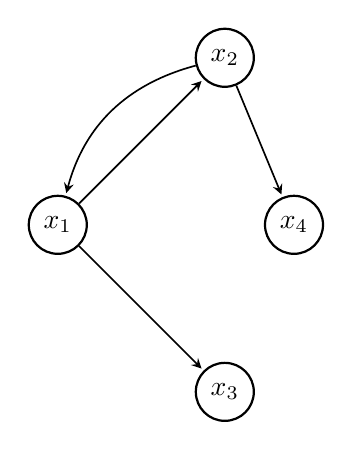
\begin{tikzpicture}[
            > = stealth, % arrow head style
            shorten > = 1pt, % don't touch arrow head to node
            auto,
            node distance = 3cm, % distance between nodes
            semithick % line style
        ]

        \tikzstyle{every state}=[
            draw = black,
            thick,
            fill = white,
            minimum size = 4mm
        ]

        \node[state] (x_1) {$x_1$};
        \node[state] (x_2) [above right of=x_1] {$x_2$};
        \node[state] (x_3) [below right of=x_1] {$x_3$};
        \node[state] (x_4) [right of=x_1] {$x_4$};
        

        \path[->] (x_1) edge node {} (x_2);
        \path[->] (x_2) edge[bend right] node {} (x_1);
        \path[->] (x_1) edge node {} (x_3);
        \path[->] (x_2) edge node {} (x_4);
      

    \end{tikzpicture}
\caption{Factorization as directed graph} \label{fig:directed_graph}
\end{figure}

We can rewrite the factorization as follows:

\begin{align*}
	p(x_1,x_2,x_3,x_4) &= p(x_1,x_4|x_2)p(x_2,x_3|x_1)\\
	&= p(x_1|x_2)p(x_4|x_2)p(x_2|x_1)p(x_3|x_1)
\end{align*}

We can now marginalize $x_1$ and $x_2$ and apply the sum and product rule at the end to get the joint probabilities:

\begin{align*}
	p(x_1) = p(x_1|x_2)p(x_2) = p(x_2, x_1)\\
	p(x_2) = p(x_2|x_1)p(x_1) = p(x_1, x_2)
\end{align*}

Therefore:

\begin{align*}
	p(x_1)p(x_2) = p(x_1,x_2)p(x_2,x_1)\\
	p(x_1, x_2) \neq p(x_1)p(x_2)
\end{align*}

Based on this contradiction the statement $X_1 \independent X_2$ does \textbf{not} hold.

\subsection*{4.2}

\begin{align*}
	X_3 \independent X_4 | X_1,X_2
\end{align*}

\textbf{Answer:}\\

In order to show that $X_3 \independent X_4 | X_1,X_2$, we have to prove that $p(x_3, x_4 | x_1, x_2) = p(x_3 | x_1, x_2)p(x_4 | x_1, x_2)$. 

We already know from the previous exercise that 

\begin{align*}
	p(x_1)p(x_2) = p(x_1,x_2)p(x_2,x_1)
\end{align*}

and based on the symmetry property we know that:

\begin{align*}
	p(x_1,x_2) = p(x_2,x_1)
\end{align*}

We can therefore replace the joint probabilities with marginal probabilities which makes it easier to prove the conditional independence:

\begin{align*}
	p(x_1,x_2) = p(x_1)\\
	p(x_1,x_2) = p(x_2)
\end{align*}

We can rewrite the statements as follows when we replace $p(x_1,x_2)$ for $p(x_1)$:

\begin{align*}
p(x_3, x_4 | x_1, x_2) = p(x_3 | x_1, x_2)p(x_4 | x_1, x_2)\\
p(x_3,x_4|x_1) = p(x_3|x_1)p(x_4|x_1)\\
p(x_3|x_1)p(x_4|x_1) = p(x_3|x_1)p(x_4|x_1)
\end{align*}

Therefore the statement $X_3 \independent X_4 | X_1,X_2$ holds.

\end{document}
